%!TEX root = ../dokumentation.tex
\chapter{ReactJS}
\label{ch:reactJS}

\section{Allgemein}

\subsection{Einführung in das Framework}

ReactJS ist eine von Facebook entwickelte JavaScript Bibliothek zur Entwicklung von Benutzeroberflächen. Im Gegensatz zu Angular ist ReactJS ein reines View-Framework. Das Framework wird unter anderem bei Facebook, Instagram, Netflix, Airbnb und dem Content Management System Wordpress eingesetzt. Es bietet einige Vorteile bei der Entwicklung von Anwendungen mit großen Benutzeroberflächen mit Daten, die sich häufig verändern. 

Das Framework ist in JavaScript geschrieben und kann mit JavaScript oder einer in JavaScript übersetzbare Sprache wie TypeScript verwendet werden.\autocites[vgl.][1\psqq]{Gackenheimer.2015}[vgl.][3\psqq]{Zeigermann.2016}

\comment{An dieser Stelle eventuell noch mehr auf das Problem eingehen.}

\subsection{Vorbereitung der Entwicklungsumgebung}



\section{Konzepte}

\subsection{Rendern von Elementen}

%ReactElement

\subsection{Komponenten}
Komponenten sind das zentrale Element in ReactJS. Sie enthalten sowohl die Logik als auch die zugehörige Anzeige. Eine Komponente kann entweder als Klasse oder als Funktion (engl. functional components) implementiert werden.  %Laut \textcite[vgl.][82\psq]{Zeigermann.2016} solle man Komponenten vorzugsweise als Funktion implementieren,  außer es soll eine nur von klassenbasierten Komponenten bereitgestelltes Feature verwendet werden. 

Die Funktion muss genau ein React-Element zurückgeben. Die implementierte Komponente trägt den gleichen Namen wie die Funktion. Die Funktion Hello in \autoref{lst:KomponenteFunktion} implementiert die Komponente Hello.

\begin{lstlisting}[caption=Beispiel einer Komponente als Funktion, label=lst:KomponenteFunktion, language=Java]
import React from 'react';
funtion Hello(){
	return <h1>Hello World</h1>;
}
\end{lstlisting}

Eine Klasse, die eine React-Komponente implementiert, muss von \textit{React.Component} erben. Zudem muss die Klasse eine Methode \textit{render()}, die ein React-Element zurückgibt, implementieren. Das \autoref{lst:KomponenteKlasse} zeigt die Implementierung der Komponente Hello als Klasse.\autocite[vgl.][80\psqq]{Zeigermann.2016}

\begin{lstlisting}[caption=Beispiel einer Komponente als Klasse, label=lst:KomponenteKlasse, language=Java]
import React from 'react';
class Hello extends React.Component{
	render() {
		return <h1>Hello World</h1>;
	}
}
\end{lstlisting}

Durch Eigenschaften (engl. Properties) lässt sich das Aussehen und Verhalten einer Komponente von außen beeinflussen. Einer Komponente können Eigenschaften (engl. Properties) in Form eines Objektes übergeben werden. Eine Veränderung der Properties durch die Komponente ist nicht möglich. Bei Komponentenfunktionen wird das Objekt der Funktion und bei Komponentenklassen dem Konstruktor der Klasse übergeben. Nach der Weitergabe des Objekts an die Oberklasse React.Component stehen die Properties über die Instanzvariable \textit{props} zur Verfügung. \autocites[vgl.][24\psq,83-88]{Zeigermann.2016}[vgl.][12-17]{Stefanov.2017}

%Die von einer Komponente erwarteten Eigenschaften können über das Objekt \textit{propTypes} beschrieben werden. Das Objekt \textit{defaultProps} ermöglicht zudem das Bestimmen von Default-Werten für die Eigenschaften. Bei Komponentenfunktionen muss das Objekt als Eigenschaft der Funktion und bei Komponentenklassen als statisches Attribut an die Klasse gesetzt werden. Dies hat den Vorteil das React diese zur Laufzeit überprüfen und eine entsprechende Warnung ausgeben kann. Zudem kann der Entwickler auf einen Blick die von einer Komponenten erwarteten Eigenschaften erkennen. 


Die Komponentenklasse bietet gegenüber der Komponentenfunktion einige zusätzliche Funktionen. Eine  Komponente, die als Klasse implementiert wird, hat einen Zustand (engl. State). Dieser wird in der Instanzvariable \textit{state} gehalten und kann nur von der Komponente gelesen und verändert werden. Die Änderung des States sollte hauptsächlich über die Methode \textit{setState()} erfolgen. Diese Methode  erwartet ein Objekt mit KeyValue-Paaren oder eine Callback-Funktion. Durch den Aufruf der Methode wird der State mit dem bisherigen State zusammengeführt.\autocites[vgl.][24\psq,89-93]{Zeigermann.2016}[vgl.][17\psq]{Stefanov.2017}

Eine Änderung an den Properties oder am State führt zum erneuten Rendern einer Komponente. Dieser Vorgang erfolgt asynchron. Änderungen werden zum Teil zusammengefasst und nicht sofort angewandt. \autocites[vgl.][24\psq, 90\psq]{Zeigermann.2016}


Eine Komponente hat einen gewissen Lebenszyklus. In diesen Zyklus kann bei Verwendung einer Komponentenklasse durch Überschreiben von Lebenszyklus-Methoden (engl. lifecycle-methods) eingegriffen werden. Die \autoref{fig:LifecyleComponent} zeigt die gebräuchlichsten Lebenszyklus-Methoden einer Komponente.\autocites[vgl.][96-100]{Zeigermann.2016}[vgl.][]{Facebook.2018}

%Beschreibung des Lebenszyklusses einer Komponente

\begin{figure}
	\centering
	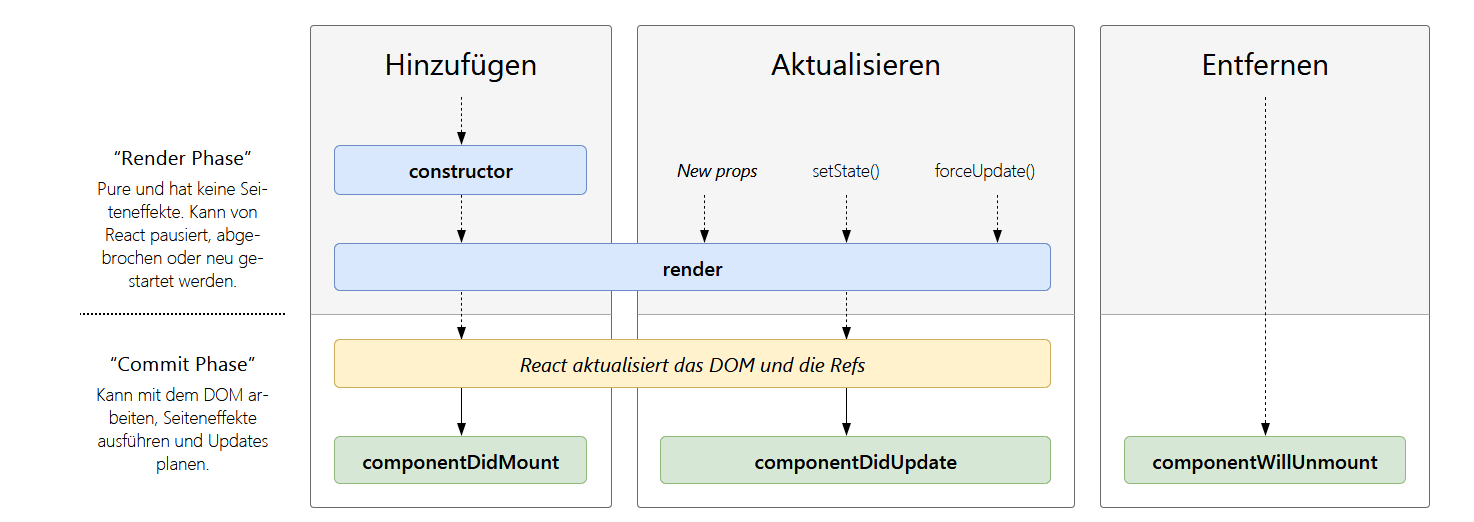
\includegraphics[width=\linewidth]{ReactLifecycle.png}
	\caption{Lebenszyklus einer  React-Komponente} 
	\quelle{\textcite{Maj.2018}}
	\label{fig:LifecyleComponent}
\end{figure}


   


  
%Auf die Zusammenarbeit der einzelnen Komponenten eingehen...Wie sieht eine typische React Anwendung aus?

\section{Verwendung}


